\documentclass{article}

% This is a comment line in latex

\usepackage[T1]{fontenc}
\usepackage[utf8]{inputenc}
\usepackage[french]{babel}

%% This package is necessary to use \includegraphics.
\usepackage{graphicx}

%% This package is necessary to define hyperlinks.
\usepackage{hyperref}

%% These packages are necessary to include code.
\usepackage{listings}
\usepackage{minted} % colored

%% This package is needed to enchance mathematical formulas.
\usepackage{amsmath}


% Latex allows you to define your own "commands",
% better known as "macros" in the Latex world.
% The following line is an example of such definition.
\newcommand{\latex}{\LaTeX}

% The next lines contain some meta informations about this document.

\title{
  Rapport intermédiaire pour \\
  ``Projet de programmation''\\
  Date d'échéance : 15 mars 2025
}


\author{Guillaume Xue et David Yu}

%% Here we begin giving the actual content o the document.
\begin{document}
\maketitle

\selectlanguage{french}

\section{Introduction}
Le but de ce projet est de développer une version personnalisée 
de \textit{Pokémon Donjon Mystère} en OCaml en mettant l'accent 
sur la génération procédurale de cartes, l'affichage des éléments 
du jeu et les interactions du joueur.

\subsection{Métriques de succès}
Le succès du projet sera mesuré à travers les critères suivants :
\begin{itemize}
    \item La génération procédurale des donjons 
    de façon cohérente et diversifiée.
    \item Fonctionnalités du menu (création et chargement de partie).
    \item Bonne gestion des collisions et animation du joueur.
    \item Stabilité et performance du jeu.
    \item Organisation en modules bien structurés.
    \item Code réutilisable et bien documenté.
\end{itemize}

\section{Implémentation}

\subsection{Développement et organisation du code}
\begin{itemize}
  \item \textbf{Module Génération de cartes} : Implémente les algorithmes (automate cellulaire, Prim, Flood fill, Voronoi).
  \item \textbf{Module Affichage} : Gère le rendu graphique du menu, du joueur et des biomes.
  \item \textbf{Module Interaction} : Assure les déplacements du joueur et les collisions avec l’environnement.
  \item \textbf{Module Gestion des données} : Stocke les statistiques du joueur et les sauvegardes de partie.
\end{itemize}

\subsection{Structure des données}
Dans notre projet, nous avons structuré les données en plusieurs catégories 
pour organiser les informations essentielles du jeu : 
\begin{itemize}
  \item Une structure pour la carte, stockée sous forme de grille de tuiles.
  \item Une structure pour le joueur, avec position, statistiques et apparence.
  \item Un regroupement des données dans une structure globale pour l’état du jeu.
  \item Un système de conversion JSON <-> OCaml pour gérer les sauvegardes.
\end{itemize}
Nous utilisons des types algébriques, des enregistrements et des structures 
adaptées à OCaml pour gérer ces éléments de manière efficace.

\subsection{Technologies utilisées}
Le projet repose sur les technologies suivantes :
\begin{itemize}
    \item Langage : OCaml
    \item Algorithmes : Automate cellulaire, algorithme de Prim, Flood fill, Voronoi
    \item Bibliothèques graphiques utilisées : Raylib
\end{itemize}

\begin{figure}
  \centering
  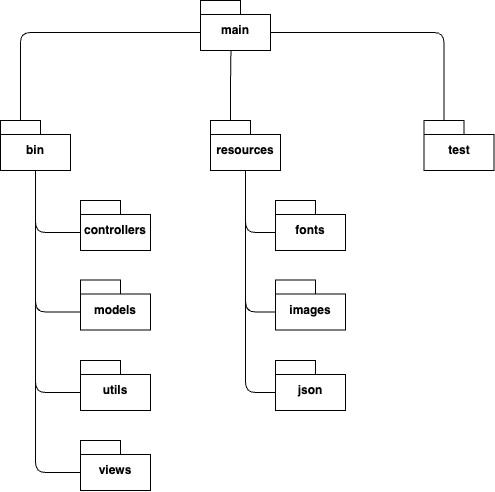
\includegraphics[width=0.8\textwidth]{structure.drawio.png}
  \caption{Schéma de la structure du projet}
\end{figure}

\section{Jalons}

\subsection{Avancement actuel}
Les tâches déjà accomplies sont :
\begin{itemize}
    \item Génération procédurale de la carte.
    \item Affichage du menu principal.
    \item Affichage du joueur et des animations.
    \item Affichage des biomes.
    \item Gestion des collisions.
    \item Affichage des statistiques du joueur.
    \item Système de sauvegarde.
\end{itemize}

\subsection{Prochaines étapes}
Les tâches à venir sont :
\begin{itemize}
    \item Génération des ennemis, obstacles et des objets.
    \item Système de combat.
    \item Système d’inventaire.
    \item Génération des boss.
    \item Amélioration de l’interface graphique.
\end{itemize}
\begin{figure}
  \centering
  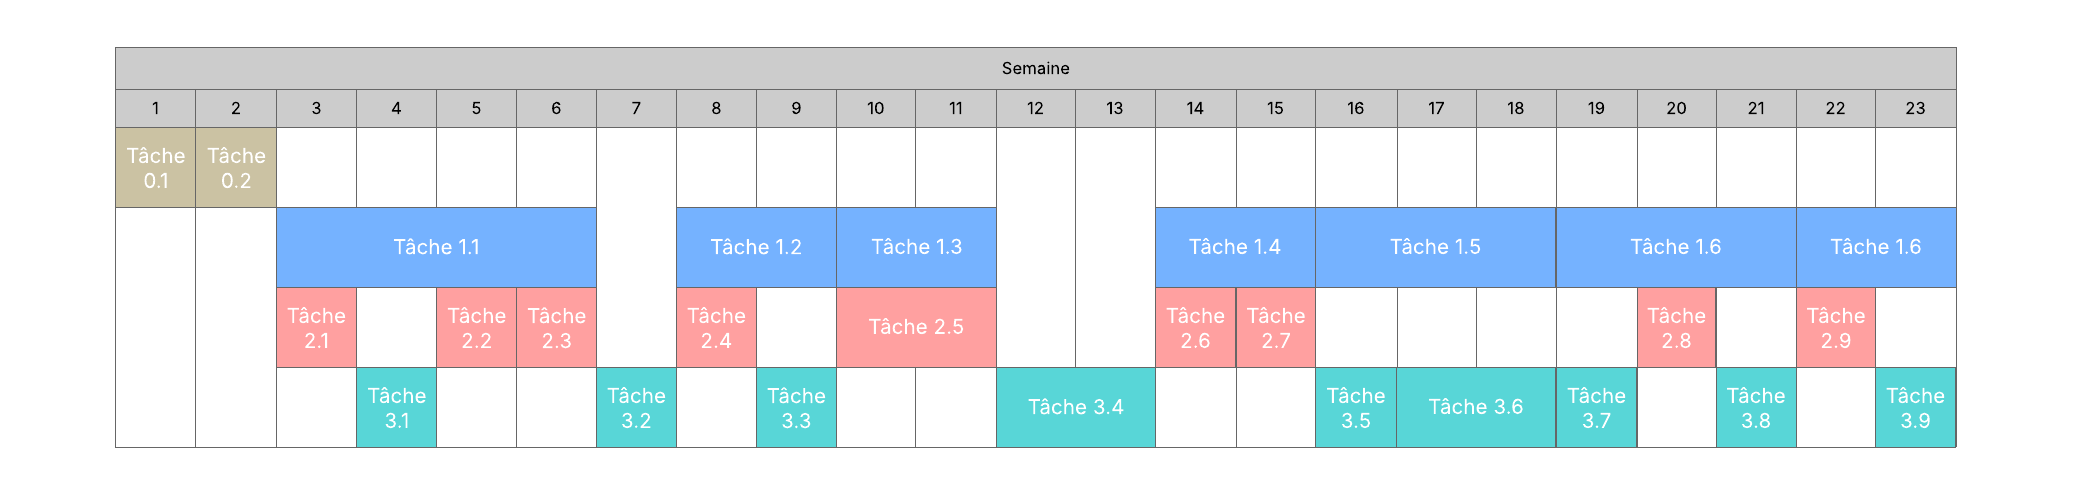
\includegraphics[width=1\textwidth]{Diagramme_de_Gantt.png}
  \caption{Diagramme de Gantt}
  \vspace{1cm}
  \begin{itemize}
    
    \item Tâche 0.1 : Définition des algorithmes de génération de carte.
    \item Tâche 0.2 : Creation de la structure du projet.

    \item Tâche 1.1 : Automate cellulaire.
    \item Tâche 1.2 : Algorithme de Prim, Flood fill.
    \item Tâche 1.3 : Algorithme de Voronoi.
    \item Tâche 1.4 : Génération des obstacles.
    \item Tâche 1.5 : Génération des ennemis.
    \item Tâche 1.6 : Génération des objets.
    \item Tâche 1.7 : Génération des boss.

    \item Tâche 2.1 : Affichage de la carte et des biomes.
    \item Tâche 2.2 : Affichage du menu principal.
    \item Tâche 2.3 : Affichage du menu de chargement nouvelle carte.
    \item Tâche 2.4 : Affichage du menu de sauvegarde.
    \item Tâche 2.5 : Affichage du joueur avec camera centrer.
    \item Tâche 2.6 : Affichage des obstacles.
    \item Tâche 2.7 : Affichage des ennemis.
    \item Tâche 2.8 : Affichage des objets et inventaire.
    \item Tâche 2.9 : Affichage des boss.

    \item Tâche 3.1 : structure du joueur.
    \item Tâche 3.2 : système de chargement.
    \item Tâche 3.3 : système de sauvegarde.
    \item Tâche 3.4 : déplacement, collision, statistiques du joueur.
    \item Tâche 3.5 : structure des ennemis.
    \item Tâche 3.6 : IA des ennemis.
    \item Tâche 3.7 : système de combat.
    \item Tâche 3.8 : système d’inventaire.
    \item Tâche 3.9 : système d’objets.
  \end{itemize}
\end{figure}


\end{document}